\setchapterpreamble[u]{\margintoc}
\chapter{The Hydrogen Atom}
\labch{intro}

This is a very common and well study problem in quantum mechanics. The hydrogen atom is the simplest atom, and it is composed by a proton and an electron. The proton is located at the origin of the coordinate system, and the electron is located at a distance $r$ from the proton. The electron is described by a wave function $\psi(r,\theta,\phi)$, and the potential energy is given by the Coulomb potential. During this chapter we will go through all the theory and compare it with the result from the experiment done in the Modern Physics Lab.


\section{The electric potential}

The electric potential is well known since the 18th century. The potential is given by:

\begin{equation}
  \begin{array}{c}
    V(r) = -\frac{1}{4\pi\epsilon_0}\frac{Ze^2}{r}
  \end{array}
\end{equation}

Where $Z$ is the atomic number of the atom, $e$ is the absolut value of the charge of the electron, and $\epsilon_0$ is the vacuum permittivity. We are also going to define $\hbar$ as the Plank's constant and $m$ as the relative mass in this case, the mass of the electron. All these values are well known and the values get better every year. These values are:

\begin{equation}
  \begin{array}{c}
    e = 1.602176634 \cdot 10^{-19} \, \text{C} \\
    \epsilon_0 = 8.8541878128 \cdot 10^{-12} \, \frac{C^2 s^2}{kg m^2} \\
    m = 9.1093837015 \cdot 10^{-31} \, \text{kg}\\
    \hbar = 1.054571817 \cdot 10^{-34} \, \frac{kg m^2}{s}
  \end{array}
\end{equation}

We are going to look at the wave equation with natural units.

\begin{equation}
  \begin{array}{c}
    r = b u
    \\

    \\
    W_{E,j}(r=bu) = \chi_{E,j}(u)
  \end{array}
\end{equation}

So the wave equation is:

\begin{equation}
  \begin{array}{c}
  \frac{1}{b^2} \frac{d^2\chi}{du^2} + \frac{2(j+1)}{b^2 u}\frac{d \chi}{du} + \left(\frac{2mE}{\hbar^2} + \frac{2m}{\hbar^2}\frac{Ze^2}{4\pi\epsilon_0}\frac{1}{ub}\right)\chi = 0
  \\

  \\
  \frac{d^2\chi}{du^2} + \frac{2(j+1)}{u} \frac{d\chi}{du} + \left(\frac{2mEb^2}{\hbar^2}+\frac{2m}{\hbar^2}\frac{Ze^2 b}{4\pi\epsilon_0}\frac{1}{u}\right)\chi = 0
  \end{array}
\end{equation}

We want to find b so the term that belongs to the potential is equal to 1.

\begin{equation}
  \begin{array}{c}
    b = \frac{2\pi \epsilon_0 \hbar^2}{Z e^2 m} = [m] = \frac{1}{Z} 2.64588603 \cdot 10^{-19} m
  \end{array}
\end{equation}

That number is the natural atomic unit for length. The natural scal, b, becomes smaller with bigger Z.

We can also define the energy in natural units.

\begin{equation}
  \begin{array}{c}
    E = -\frac{\hbar^2}{2mb^2}\alpha
  \end{array}
\end{equation}

Where alpha can be either positive or negative. The wave equation looks like:

\begin{equation}
  \begin{array}{c}
    \frac{d^2\chi}{du^2} + \frac{2(j+1)}{u}\frac{d\chi}{du}-\alpha\chi +\frac{1}{u}\chi= 0
  \end{array}
\end{equation}

When u goes to infinite the equation become:

\begin{equation}
  \begin{array}{c}
    \frac{d^2\chi}{du^2} = \alpha\chi \rightarrow \chi = C_1 e^{-\sqrt{\alpha}u} - C_2 e^{\sqrt{\alpha}u}
  \end{array}
\end{equation}

Since $\chi$ has to go to 0 when $u$ goes to infinite, because of the normalization condition, $C_2$ is going to be 0 and alpha has to be postive, sowe can rewrite this in terms of:

\begin{equation}
  \begin{array}{c}
    \alpha=\beta^2
    \\

    \\
    E = -\frac{Z^2e^4m}{8\pi^2\epsilon_0^2\hbar^2}\beta^2
    \\

    \\
    \chi(u) = e^{-\beta u}R(u)
  \end{array}
\end{equation}

We are going to find the different terms in the wave equation separatly.

\begin{equation}
  \begin{array}{c}
    \frac{d^2\chi}{du^2} = \beta^2 e^{-\beta u} R - 2\beta e^{-\beta u} \frac{dR}{du}+e^{-\beta u} \frac{d^2R}{du^2}
    \\

    \\
    \frac{2(j+1)}{u} \frac{d\chi}{du} = \frac{-2(j+1)}{u} e^{\beta u} R + \frac{2(j+1)}{u} e^{\beta u} \frac{dR}{du}
    \\

    \\
    \left(\frac{1}{u}-\beta^2\right)\chi = \frac{1}{u} e^{\beta u}R -e^{\beta u} R
  \end{array}
\end{equation}

So the wave equation looks like:

\begin{equation}
  u\frac{d^2R}{du^2}+(2(j+1)-2\beta u)\frac{dR}{du} + (1 - 2(j+1)\beta)R = 0
\end{equation}

We can solve this differential equation using the power series method. We are going to assume that the solution is a power series.

\begin{equation}
  \begin{array}{c}
    R(u) = \sum_{k=0}^{\infty} C_k u^k
    \\

    \\
    \frac{dR}{du} = \sum_{k=0}^{\infty} C_{k+1} (k+1) u^{k}
    \\

    \\
    \frac{d^2R}{du^2} = \sum_{k=0}^{\infty} C_{k+1} k(k+1) u^{k-1}
  \end{array}
\end{equation}

We can substitute this into the wave equation, trying to match the indices of all the terms to the same $u^{k}$ and we get:

\begin{equation}
  \begin{array}{c}
    \sum_{k=0}^{\infty} C_{k+1} k (k+1) u^k +
    \\

    \\
    \sum_{k=0}^{\infty} C_{k+1} (k+1) 2(j+1) u^k -
    \\

    \\
    \sum_{k=0}^{\infty} C_{k} 2\beta k u^k +
    \\

    \\
    \sum_{k=0}^{\infty} C_{k} (1-2(j+1)\beta) u^k = 0
    \\

    \\
    \sum_{k=0}^{\infty} u^k\left[C_{k+1}\left[k(k+1)+2(k+1)(j+1)\right]+ \right.
    \\

    \\
    \left. C_k \left[ 1-2(j+1)\beta-2\beta k \right]\right] = 0
    \\

    \\
    C_k+1 =\frac{2\beta k-1+2\beta(j+1)}{(k+1)(k+2(j+1))}C_k = \frac{2\beta (k+j+1)}{(k+1)(k+2(j+1))} C_k
  \end{array}
\end{equation}

The power serie has to be finite because the $R_E,j(u)$ has to be normaliable. This means that for some k=p the coefficient $C_{p+1}$ has to be 0.

\begin{equation}
  \begin{array}{c}
    2\beta (p+j+1) -1 = 0
    \\

    \\
    \beta = \frac{1}{2(p+j+1)} = \frac{1}{2n}
  \end{array}
\end{equation}

Where n is $n=p+j+1$. Because p and j are define as integer numbers from 0 to infinte, n is an integer number, but from 1 to infinite. Now we can define the energy in terms of n.

\begin{equation}
  \begin{array}{c}
    E = -\frac{Z^2 e^4 m}{32\pi^2\epsilon_0^2\hbar^2 n^2}
  \end{array}
\end{equation}

That is the energy for the eigen-functions:

\begin{equation}
  \begin{array}{c}
    \psi_{n,j,m} = \left(\sum_{k=0}^{n-j-1} C_k u^k \right)e^{-\frac{1}{2n}u}(bu)P_j^m(\theta)e^{im\phi}
  \end{array}
\end{equation}

We can plot some of the eigen-functions to see how they look like.

\section{Eigen-functions of the hydrogen atom}


\begin{figure}
  \centering
  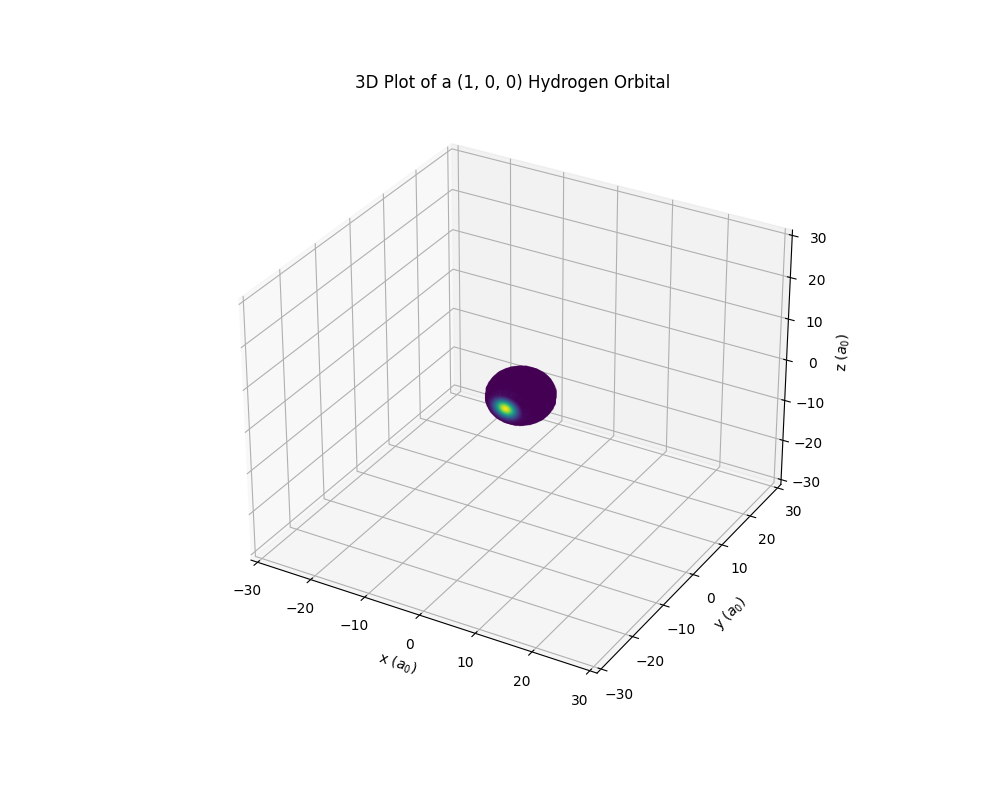
\includegraphics{images9/3d_plot_1,0,0.png}
  \caption{Probability distribution (n=1,j=0,m=0)}
\end{figure}

\begin{figure}
  \centering
  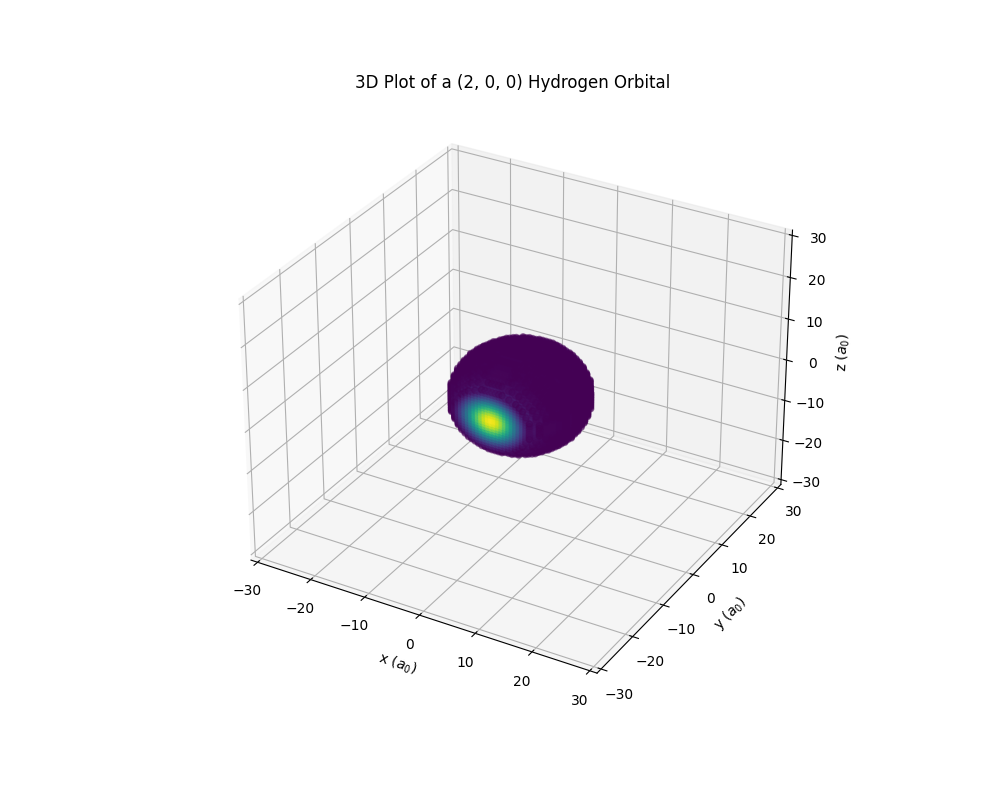
\includegraphics{images9/3d_plot_2,0,0.png}
  \caption{Probability distribution (n=2,j=0,m=0)}
\end{figure}

\begin{figure}
  \centering
  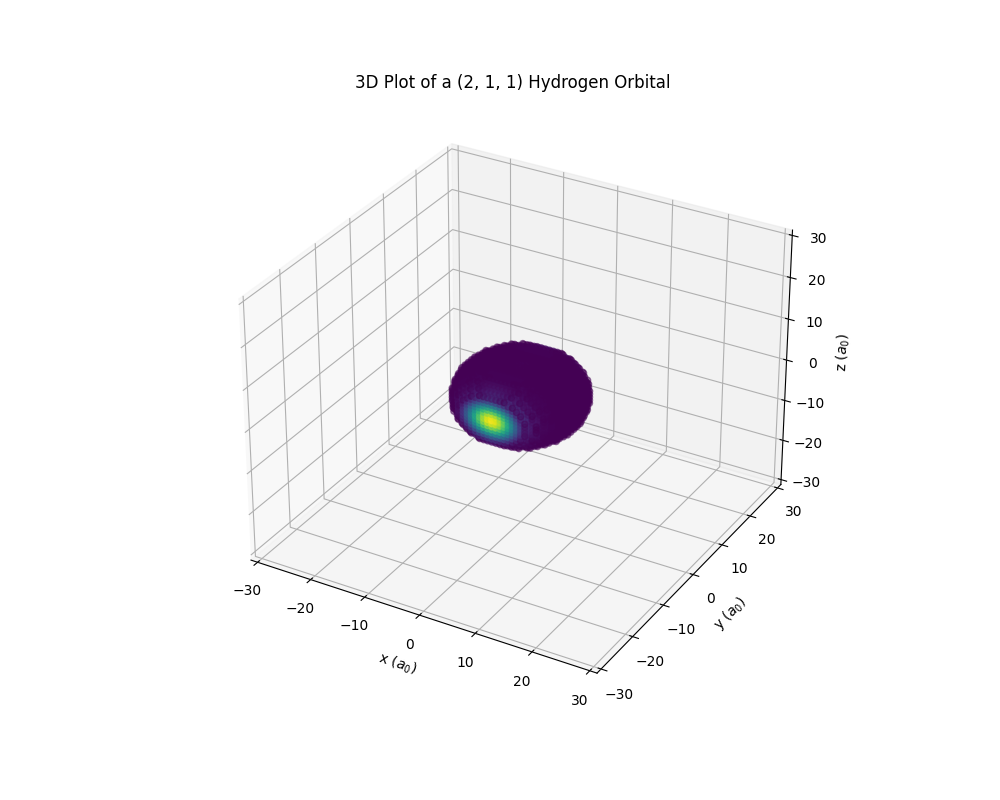
\includegraphics{images9/3d_plot_2,1,1.png}
  \caption{Probability distribution (n=2,j=1,m=1)}
\end{figure}

\begin{figure}
  \centering
  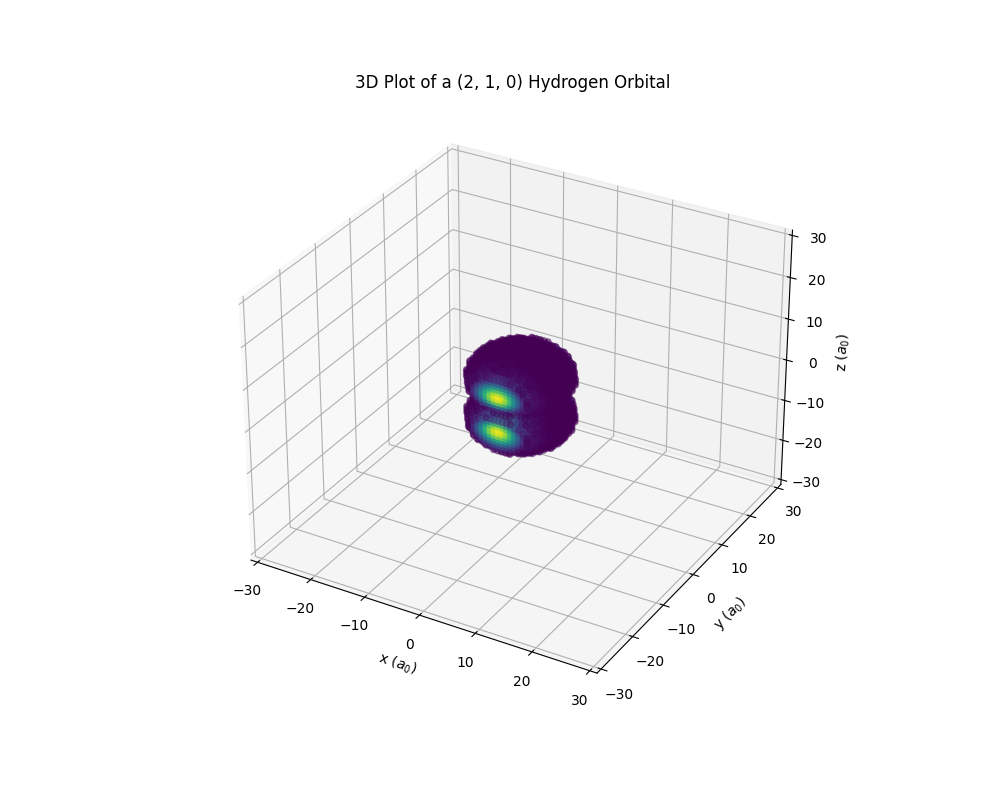
\includegraphics{images9/3d_plot_2,1,0.png}
  \caption{Probability distribution (n=2,j=1,m=0)}
\end{figure}

\begin{figure}
  \centering
  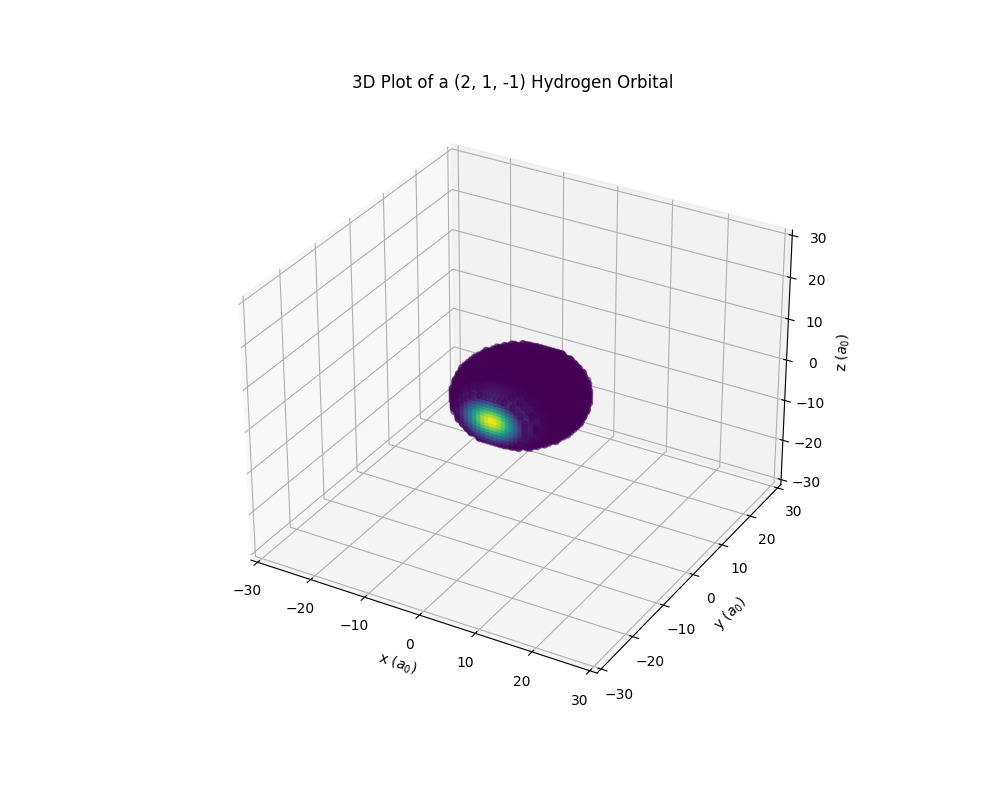
\includegraphics{images9/3d_plot_2,1,-1.png}
  \caption{Probability distribution (n=2,j=1,m=-1)}
\end{figure}


\section{Temperature and Light}

If we look at the plot of  the energy depending on n,we are going to see that the gap between the first energies is bigger than those of the higher energies. To move from one energy level to a higer one we need some temperature. The energy needed to move from the energy $E_i$ to $E_f$ is determined by the factor $KT$, where $K$ is the Boltzmann constant and $T$ is the temperature.

\begin{equation}
  \begin{array}{c}
    \Delta E = E_f - E_i = KT
  \end{array}
\end{equation}

This means that if the temperature is higher we will be able to reach higher energies. However the probability of the particle to be in the lowest energy is always greater or equal than the energy of the particle to be in a higher energy level. This is given by the Boltzmann distribution.

\begin{equation}
  \begin{array}{c}
    P(E_n) \propto e^{-\frac{E_n}{KT}}
  \end{array}
\end{equation}

In the same way we can see that energy can be emitted from the electron when it change from a higher energy to a lower energy state. This energy is going to be emitted in the form of light. The energy of the light is going to be the same as the energy difference between the two energy levels.

\begin{equation}
  \begin{array}{c}
    \Delta E = E_f - E_i = h\omega_{light}
  \end{array}
\end{equation}


\section{The relativistic wave equation.}

We are going to start this section with the question of what happens if j is not an integer number. We are going to need a new approach to answer this question because we are basing all our calculations in the fact that m is an integer because there is a symmetry in the problem, $(f(\phi)=f(\phi+2\pi))$.

For this new aproach we are going to redefine the energy using what we know from relativity.

\begin{equation}
  \begin{array}{c}
    E^2 = p^2c^2 + m^2c^4
  \end{array}
\end{equation}

Let's try to find the wave equation using this relation for one dimension.

\begin{equation}
  \begin{array}{c}
   \left[-\hbar^2\frac{d^2}{dt^2}\right]\psi(x,t) = \left[- \hbar^2c^2\frac{d^2}{dx^2}+m^2c^4\right]\psi(x,t)
  \end{array}
\end{equation}

We can not really solve this equation with the knowledge we have, let's talk about something first.

\section{Pauli matrices}

If we look at the matrices of the angular momentum for j=1/2 in equation \ref{9.48} we can rewrite them as:

\begin{equation}
  L_a =\frac{\hbar}{2} \sigma_a
\end{equation}

Where $\sigma_a$ are the Pauli matrices. The Pauli matrices are defined as:

\begin{equation}
  \sigma_1 = \begin{pmatrix}
    0 & 1 \\
    1 & 0
  \end{pmatrix},
  \sigma_2 = \begin{pmatrix}
    0 & i \\
    -i & 0
  \end{pmatrix},
  \sigma_3 = \begin{pmatrix}
    -1 & 0 \\
    0 & 1
  \end{pmatrix}
\end{equation}

We can test their properties.

\begin{equation}
  \begin{array}{c}
    \left[L_a,L_b\right] = \frac{\hbar^2}{4} \left[\sigma_a,\sigma_b\right] = i\frac{\hbar^2}{2}\epsilon_{a,b,c}\sigma_c
    \\

    \\
    \left[\sigma_a,\sigma_b\right] = 2i \epsilon_{a,b,c}\sigma_c
  \end{array}
\end{equation}

And we can observed from \ref{9.49} that:
\begin{equation}
  \sigma_a^2 = \mathbb{1}
\end{equation}

Other intweresting property pf the Pauli matrices is:

\begin{equation}
  \begin{array}{c}
    \sigma_1 \sigma_2 = i\sigma_3
    \\
    \sigma_2 \sigma_1 = -i\sigma_3
    \\
    \sigma_2 \sigma_3 = i\sigma_1
    \\
    \sigma_3 \sigma_2 = -i\sigma_1
    \\
    \sigma_3 \sigma_1 = i\sigma_2
    \\
    \sigma_1 \sigma_3 = -i\sigma_2
  \end{array}
\end{equation}

In general we can say two things. The first one is that the anticonmmutation is 0, where we define the anticonmmutation as:

\begin{equation}
  {A,B} = AB+BA
\end{equation}

And also, the general multiplication of any two terms of the matrices is defined as:

\begin{equation}
\begin{array}{c}
  \sigma_a \sigma_b = \delta_{a,b}\mathbb{1} + i\epsilon_{a,b,c}\sigma_c
\end{array}
\end{equation}

\section{The Dirac operator}

We are going to try to solve the relativistic wave equation in one dimension. For that we are going to define D-slash as:

\begin{equation}
  \begin{array}{c}
    (\slashed{D})^2 = -\hbar^2 \frac{\partial^2}{\partial t^2} + \hbar^2 c^2 \frac{\partial^2}{\partial x^2}
    \\

    \\
    \slashed{D} = i\hbar\gamma_0 \frac{\partial}{\partial t}-i\hbar c \gamma_1 \frac{\partial}{\partial x}
    \\

    \\
    (\slashed{D})^2 = \left(i\hbar\gamma_0\frac{\partial}{\partial t}-i\hbar c\gamma_1\frac{\partial}{\partial x}\right)\left(i\hbar\gamma_0\frac{\partial}{\partial t}-i\hbar c\gamma_1\frac{\partial}{\partial x}\right)
    \\

    \\
    (\slashed{D})^2 = -\hbar^2 \gamma_0^2 \frac{\partial^2}{\partial t^2} + \hbar^2 c^2 \gamma_1^2 \frac{\partial^2}{\partial x^2} + \hbar^2 c (\gamma_0\gamma_1 + \gamma_1\gamma_0)\frac{\partial^2}{\partial t \partial x}
  \end{array}
\end{equation}

We want to find this  gamma matrices following the next rules.

\begin{equation}
  \begin{array}{c}
    \\
    \gamma_0^2 = \mathbb{1}
    \\
    \gamma_1^2 = -\mathbb{1}
    \\
    \gamma_0\gamma_1 + \gamma_1\gamma_0 = 0
  \end{array}
\end{equation}

This look similar to the conditions of the Pauli matrices. So we can say that:

\begin{equation}
  \begin{array}{c}
    \gamma_0 = \sigma_1
    \\
    \gamma_1 = i\sigma_2
  \end{array}
\end{equation}

D-slash looks like:

\begin{equation}
  \begin{array}{c}
    \slashed{D} = i\hbar\begin{bmatrix}
      0 & 1\\
      1 & 0\end{bmatrix} \frac{\partial}{\partial t} + \hbar c \begin{bmatrix}
      0 & i\\
      -i & 0\end{bmatrix} \frac{\partial}{\partial x} =
      \\

      \\
      = \begin{bmatrix}
      0 & i\hbar c \frac{\partial}{\partial x} + \hbar \frac{\partial}{\partial t}\\
      i\hbar \frac{\partial}{\partial t} - i\hbar c \frac{\partial}{\partial x} & 0\end{bmatrix}
  \end{array}
\end{equation}

Now we can extend this to two dimensions.

\begin{equation}
  \begin{array}{c}
  \slashed{D} = i\hbar\gamma_0 \frac{\partial}{\partial t} - i\hbar c \gamma_1 \frac{\partial}{\partial x} - i\hbar c\gamma_2 \frac{\partial}{\partial y}
  \\

  \\
  \begin{array}{llll}
    (\slashed{D})^2 &= -\hbar^2 \gamma_0^2 \frac{\partial^2}{\partial t^2} &+ \hbar^2 c^2 \gamma_1^2 \frac{\partial^2}{\partial x^2} &+ \hbar^2 c (\gamma_0\gamma_1 + \gamma_1\gamma_0)\frac{\partial^2}{\partial t \partial x}
    \\

    \\
                    &+ \hbar^2 c (\gamma_1\gamma_2 + \gamma_2\gamma_1)\frac{\partial^2}{\partial x \partial y}  &+\hbar^2 c^2 \gamma_2^2 \frac{\partial^2}{\partial y^2}  &+ \hbar^2 c (\gamma_0\gamma_2 + \gamma_2\gamma_0)\frac{\partial^2}{\partial t \partial y}
  \end{array}
\end{array}
\end{equation}

With the new conditions.

\begin{equation}
\begin{array}{c}
  \gamma_2 =i\sigma_3
\end{array}
\end{equation}

And D-slash looks like:

\begin{equation}
  \begin{array}{c}
    \slashed{D} = \begin{bmatrix}
      -\hbar c \frac{\partial}{\partial y} &  i\hbar \frac{\partial}{\partial t}+i\hbar c\frac{\partial}{\partial x} \\
      i\hbar \frac{\partial}{\partial t}-i\hbar c\frac{\partial}{\partial x} & \hbar c \frac{\partial}{\partial y}\end{bmatrix}
  \end{array}
\end{equation}

Since now we've been defining the Dirac's operator as a 2x2 matrix, but in 3D we are going to need something different.

\begin{equation}
  \begin{array}{c}
    \slashed{D} = i\hbar\gamma_0 \frac{\partial}{\partial t} - i\hbar c \gamma_1 \frac{\partial}{\partial x} - i\hbar c\gamma_2 \frac{\partial}{\partial y} - i\hbar c\gamma_3 \frac{\partial}{\partial z}
    \\

    \\
    \begin{array}{llll}
      (\slashed{D})^2 &= -\hbar^2 \gamma_0^2 \frac{\partial^2}{\partial t^2} &+ \hbar^2 c^2 \gamma_1^2 \frac{\partial^2}{\partial x^2} &+ \hbar^2 c (\gamma_0\gamma_1 + \gamma_1\gamma_0)\frac{\partial^2}{\partial t \partial x}
    \\

    \\
                    &+ \hbar^2 c (\gamma_1\gamma_2 + \gamma_2\gamma_1)\frac{\partial^2}{\partial x \partial y}  &+\hbar^2 c^2 \gamma_2^2 \frac{\partial^2}{\partial y^2}  &+ \hbar^2 c (\gamma_0\gamma_2 + \gamma_2\gamma_0)\frac{\partial^2}{\partial t \partial y}
    \\

    \\
                    &+\hbar^2 c (\gamma_1\gamma_3 + \gamma_3\gamma_1)\frac{\partial^2}{\partial x \partial z}  &+\hbar^2 c^2 \gamma_3^2 \frac{\partial^2}{\partial z^2} &+ \hbar^2 c (\gamma_0\gamma_3 + \gamma_3\gamma_0)\frac{\partial^2}{\partial t \partial z}
    \\

    \\
                    &+\hbar^2 c (\gamma_2\gamma_3 + \gamma_3\gamma_2)\frac{\partial^2}{\partial y \partial z}
    \end{array}
  \end{array}
\end{equation}

We don't have enough Pauli matrices this time to cover all the conditions. The very clever solution to this problem was saying that D-slash is not a 2x2 matrix but a 4x4 where the gamma factors are:

\begin{equation}
  \label{10.37}
\begin{array}{c}
  \gamma_0 = \begin{bmatrix}
    \mathbb{1} & 0\\
    0 & -\mathbb{1}
  \end{bmatrix}
  \\

  \\
  \gamma_a = \begin{bmatrix}
    0 & -\sigma_a\\
    \sigma_a & 0
  \end{bmatrix}
\end{array}
\end{equation}

Where a is 1,2,3. We can see that the gamma matrices are 4x4 matrices. We can also see that the gamma matrices are hermitian and that they satisfy the anticonmmutation relation, but we want to make sure that we didn't make any mistakes.

\begin{equation}
  \gamma_0^2 = \begin{bmatrix}
    \mathbb{1} & 0\\
    0 & -\mathbb{1}
  \end{bmatrix}\begin{bmatrix}
    \mathbb{1} & 0\\
    0 & -\mathbb{1}
  \end{bmatrix} = \begin{bmatrix}
    \mathbb{1} & 0\\
    0 & \mathbb{1}
  \end{bmatrix} = \mathbb{1}_{4x4}
\end{equation}

\marginnote[-1cm]{I choose to call $\mathbb{1}$ to the 2x2 identity matrix and $\mathbb{1}_{4x4}$ to the 4x4 identity matrix.}

\begin{equation}
  \gamma_a^2 = \begin{bmatrix}
    0 & -\sigma_a\\
    \sigma_a & 0
  \end{bmatrix}\begin{bmatrix}
    0 & -\sigma_a\\
    \sigma_a & 0
  \end{bmatrix} = \begin{bmatrix}
    -\sigma_a^2 & 0\\
    0 & -\sigma_a^2\end{bmatrix} = - \mathbb{1}_{4x4}
\end{equation}

\begin{equation}
  \begin{array}{c}
    \gamma_a\gamma_0 + \gamma_0\gamma_a =
    \\

    \\
    \begin{bmatrix}
      0 & -\sigma_a\\
      \sigma_a & 0
    \end{bmatrix}\begin{bmatrix}
      \mathbb{1} & 0\\
      0 & -\mathbb{1}
    \end{bmatrix} +
    \begin{bmatrix}
      \mathbb{1} & 0\\
      0 & -\mathbb{1}
    \end{bmatrix}\begin{bmatrix}
      0 & -\sigma_a\\
      \sigma_a & 0
    \end{bmatrix} =
    \\

    \\
    \begin{bmatrix}
      0 & -\sigma_a\\
      -\sigma_a & 0
    \end{bmatrix} +
    \begin{bmatrix}
      0 & \sigma_a\\
      \sigma_a & 0
    \end{bmatrix} = 0
  \end{array}
\end{equation}

\begin{equation}
  \begin{array}{c}
    \gamma_a\gamma_b + \gamma_b\gamma_a =
    \\

    \\
    \begin{bmatrix}
      0 & -\sigma_a\\
      \sigma_a & 0
    \end{bmatrix}\begin{bmatrix}
      0 & -\sigma_b\\
      \sigma_b & 0
    \end{bmatrix} + \begin{bmatrix}
      0 & -\sigma_b\\
      \sigma_b & 0
    \end{bmatrix}
    \begin{bmatrix}
      0 & -\sigma_a\\
      \sigma_a & 0
    \end{bmatrix} =
    \\

    \\
    = \begin{bmatrix}
      -\sigma_a\sigma_b & 0\\
      0 & -\sigma_b\sigma_a
    \end{bmatrix}+ \begin{bmatrix}
      -\sigma_b\sigma_a & 0\\
      0 & -\sigma_a\sigma_b
    \end{bmatrix} =
    \\

    \\
    = -\begin{bmatrix}
      \sigma_a\sigma_b + \sigma_b\sigma_a& 0\\
      0 & \sigma_a\sigma_b + \sigma_b\sigma_a
    \end{bmatrix} = 0
  \end{array}
\end{equation}

The solution for the relativistic wave equation is going to be:

\begin{equation}
  \begin{array}{c}
    (\slashed{D})^2 \psi = m^2c^2\psi
    \\

    \\
    \slashed{D} = \pm m c^2
  \end{array}
\end{equation}

We are going to keep only the solution with the positive sign, the other one is not relevant, it can be achive just adding a minus sign to the operator.

\marginnote{Dirac's work was first called Dirac Wave Mechanics, lately this name we will be changed to Quantum Field Theory, but we are not going that far.}

The final equation in matrix form is:

\begin{equation}
  \begin{array}{c}
    (\slashed{D}-mc^2)\psi =
    \\

    \\
    = \begin{bmatrix}
      \mathbb{1} i\hbar \frac{\partial }{\partial t} - mc^2 \mathbb{1} & i\hbar c\sum_{a=1}^{3}\left(\sigma_a\frac{\partial}{\partial x_a}\right)\\
      -i\hbar c\sum_{a=1}^{3}\left(\sigma_a\frac{\partial}{\partial x_a}\right) & -\mathbb{1} i\hbar \frac{\partial }{\partial t} - mc^2 \mathbb{1}
    \end{bmatrix}\begin{bmatrix}
      \psi_1(x_1,x_2,x_3,t)\\
      \psi_2(x_1,x_2,x_3,t)\\
      \psi_3(x_1,x_2,x_3,t)\\
      \psi_4(x_1,x_2,x_3,t)
    \end{bmatrix} = 0
  \end{array}
\end{equation}

We've been using the matrices for angular momentum corresponding to j=1/2, but we haven't talk about angular momentum. Is just a coincidence.

As every other operator, we want the Dirac operator to be hermitian. We can see that the Dirac operator is not, we can see this using the properties from the end of chapter 6.

\begin{equation}
  \slashed{D}^{\dagger} = i\hbar \gamma_0 \frac{\partial}{\partial t} + i\hbar c \left(\gamma_1 \frac{\partial}{\partial x}+\gamma_2 \frac{\partial}{\partial y}+\gamma_3 \frac{\partial}{\partial z}\right)
\end{equation}

We can see that the Dirac operator is not hermitian, but we can make it hermitian by adding a term to it.

\begin{equation}
  \begin{array}{c}
  \gamma_0\slashed{D}\gamma_0 = i\hbar \gamma_0^3\frac{\partial}{\partial t} - i\hbar c\left[\gamma_0\gamma_1\gamma_0 \frac{\partial}{\partial x}+\gamma_0\gamma_2\gamma_0 \frac{\partial}{\partial y}+\gamma_0\gamma_3\gamma_0 \frac{\partial}{\partial z}\right] =
  \\

  \\
  = i\hbar \gamma_0\frac{\partial}{\partial t} + i\hbar c\left[\gamma_1 \frac{\partial}{\partial x}+\gamma_2 \frac{\partial}{\partial y}+\gamma_3 \frac{\partial}{\partial z}\right] = \slashed{D}^\dagger
  \\

  \\
  \slashed{D}\gamma_0 = \gamma_0\slashed{D}^\dagger = (\slashed{D}\gamma_0)^\dagger
  \end{array}
\end{equation}

Now we try to solve the wave equation.

\begin{equation}
\begin{array}{c}
  \gamma_0(\slashed{D}-mc^2)\psi(x,y,z,t) = 0
  \\

  \\
  \begin{bmatrix}
    \mathbb{1} & 0\\
    0 & -\mathbb{1}
  \end{bmatrix}\begin{bmatrix}
    (i\hbar \frac{\partial }{\partial t} - mc^2)\mathbb{1} & i\hbar c\sum_{a=1}^{3}\left(\sigma_a\frac{\partial}{\partial x_a}\right)\\
    -i\hbar c\sum_{a=1}^{3}\left(\sigma_a\frac{\partial}{\partial x_a}\right) & (-i\hbar \frac{\partial }{\partial t} - mc^2)\mathbb{1}
  \end{bmatrix}
  \begin{bmatrix}
    \psi_L\\
    \psi_R\\
  \end{bmatrix} = 0
  \\

  \\
  \begin{bmatrix}
    (i\hbar \frac{\partial }{\partial t} - mc^2)\mathbb{1} & i\hbar c\sum_{a=1}^{3}\left(\sigma_a\frac{\partial}{\partial x_a}\right)\\
    i\hbar c\sum_{a=1}^{3}\left(\sigma_a\frac{\partial}{\partial x_a}\right) & (i\hbar \frac{\partial }{\partial t} + mc^2)\mathbb{1}
  \end{bmatrix}
  \begin{bmatrix}
    \psi_L\\
    \psi_R\\
  \end{bmatrix} = 0
\end{array}
\end{equation}

\begin{equation}
  \begin{array}{c}
    i\hbar \mathbb{1} \frac{\partial \psi_L}{\partial t} - mc^2\psi_L + i\hbar c \left[\sigma_1\frac{\partial \psi_R}{\partial x}+\sigma_2\frac{\partial \psi_R}{\partial y}+\sigma_3\frac{\partial \psi_R}{\partial z}\right] = 0
    \\

    \\
    i\hbar c\left(\sigma_1 \frac{\partial \psi_L}{\partial x} + \sigma_2 \frac{\partial \psi_L}{\partial y}+ \sigma_3 \frac{\partial \psi_L}{\partial z}\right) \psi_L + i\hbar \mathbb{1} \frac{\partial \psi_R}{\partial t} + mc^2\psi_R = 0
  \end{array}
\end{equation}

All the components are couple, 4 eq with 4 couple terms. This system is hard to solve so we are going to guess the solution.

\begin{equation}
  \begin{array}{c}
    \psi_L = \chi_L e^{\frac{i}{\hbar}(p_1 x + p_2 y + p_3 z - Et)}
    \\

    \\
    \psi_R = \chi_R e^{\frac{i}{\hbar}(p_1 x + p_2 y + p_3 z - Et)}
  \end{array}
\end{equation}

Substituying in the previous system:

\begin{equation}
  \begin{array}{c}
    \left[E\chi_L - mc^2\chi_L- c\left(\sigma_1 p_1 + \sigma_2 p_2 + \sigma_3 p_3\right)\chi_L\right]e^{\frac{i}{\hbar}(p_1 x + p_2 y + p_3 z - Et)} = 0
    \\

    \\
    \left[-c\left( \sigma_1 p_1 + \sigma_2 p_2 + \sigma_3 p_3 \right)\chi_L + E\chi_R+ mc^2\chi_R\right] e^{\frac{i}{\hbar}(p_1 x + p_2 y + p_3 z - Et)} = 0
  \end{array}
\end{equation}

\begin{equation}
  \begin{array}{c}
    \ref{10.49}
    (E-mc^2) \chi_L = c (\sigma_1 p_1 + \sigma_2 p_2 + \sigma_3 p_3)\chi_R
    \\

    \\
    (E+mc^2) \chi_R = c (\sigma_1 p_1 + \sigma_2 p_2 + \sigma_3 p_3)\chi_L
  \end{array}
\end{equation}

To solve the system we are going to multiply by the right factor.

\begin{equation}
  \begin{array}{c}
    c(\sigma_1 p_1 + \sigma_2 p_2 + \sigma_3 p_3)(E-mc^2) \chi_L = c^2 (\sigma_1 p_1 + \sigma_2 p_2 + \sigma_3 p_3)^2\chi_R
    \\

    \\
    (E-mc^2)(E+mc^2) \chi_R = c^2 (\sigma_1 p_1 + \sigma_2 p_2 + \sigma_3 p_3)^2\chi_R
  \end{array}
\end{equation}

The matrix of the right side looks like:

\begin{equation}
  \begin{array}{c}
    \sigma_1 p_1 + \sigma_2 p_2 + \sigma_3 p_3 = \begin{bmatrix}
      -p_3 & p_1 + ip_2\\
      p_1 - ip_2 & -p_3
      \end{bmatrix}
    \\

    \\
    (\sigma_1 p_1 + \sigma_2 p_2 + \sigma_3 p_3)^2 = \begin{bmatrix}
    -p_3 & p_1 + ip_2\\
    p_1 - ip_2 & -p_3
    \end{bmatrix}\begin{bmatrix}
    -p_3 & p_1 + ip_2\\
    p_1 - ip_2 & -p_3
    \end{bmatrix} = \begin{bmatrix}
    p_1^2 + p_2^2 + p_3^2 & 0\\
    0 & p_1^2 + p_2^2 + p_3^2
    \end{bmatrix} =
    \\

    \\
    = \mathbb{1} p^2
  \end{array}
\end{equation}

The final equation is:

\begin{equation}
  \begin{array}{c}
    (E^2-m^2c^4)\chi_R = c^2 p^2\chi_R
    \\

    \\
    \begin{bmatrix}
      E^2-p^2c^2-m^2c^4 & 0\\
      0 & E^2-p^2c^2-m^2c^4
    \end{bmatrix}
    \begin{bmatrix}
      \chi_R_1\\
      \chi_R_2
    \end{bmatrix} = 0
  \end{array}
\end{equation}

Because $\chi_{R1}$ and $\chi_{R2}$ are not 0, the components of the matrix has to be 0.

\begin{equation}
  \label{10.54}
  \begin{array}{c}
    E^2 - p^2c^2 -m^2c^4 = 0
  \end{array}
\end{equation}

This means that the solution for the energy is:

\begin{equation}
  \left\{
  \begin{array}{l}
    E = + \sqrt{m^2c^4 + p^2c^2}
    \\

    \\
    E = - \sqrt{m^2c^4 + p^2c^2}
  \end{array}
  \right.
\end{equation}

We have two possible energies, both positive and negative energies are allowed, we will talk about this later.

\begin{marginfigure}
  \begin{tikzpicture}
  \draw[-] (-2,0) -- (2,0); % x-y axis
  \draw[-] (0,-2) -- (0,2); % z axis
  \filldraw[black] (2,0) circle (0pt) node [anchor=north]{$\chi_{R1}$};
  \filldraw[black] (0,2) circle (0pt) node [anchor=east]{$\chi_{R2}$};

  %vector
  \draw[->] (0,0) -- (1.5,1.5);
  \filldraw[black] (1.5,1.5) circle (0pt) node [anchor=south]{$\vec{X_R}$};

  \end{tikzpicture}
  \caption{$\chi_R$ representation}
  \labfig{chi_R}
\end{marginfigure}

Because the matrix is 0 the vector $X_R$ is going to be:

\begin{equation}
  \chi_R = \begin{bmatrix}
    1\\
    0
  \end{bmatrix} + \begin{bmatrix}
    0\\
    1
  \end{bmatrix}
\end{equation}




It started as a classical assumption but now is part of the wave equation. $\chi_R$ is a vector with two components, but is not in time or space. However they have a conection wiht j=1/2, is what we called the space of internal spin and it becames a new degree of freedom for the wave.

We still need to get $\chi_L$, let's move back to eq. \ref{10.50}, but this time we will write it as a matrix.

\begin{equation}
\begin{bmatrix}
  E-mc^2 & -c(\sigma_i p_i)\\
  -c(\sigma_i p_i) & E+mc^2
\end{bmatrix}
\begin{bmatrix}
  \chi_L\\
  \chi_R
\end{bmatrix} = 0
\end{equation}

\marginnote[-1cm]{We are using the notation $(\sigma_i p_i)$ to represent the sum of the three components of the momentum times the respective sigma matrices.}

We can do the same as before:

\begin{equation}
  \begin{array}{c}
   (E+mc^2)\chi_R = c(\sigma_i p_i)\chi_L
    \\

    \\
    (E+mc^2)c(\sigma_i p_i) \chi_R = c^2(\sigma_i p_i)^2\chi_L
  \end{array}
\end{equation}

From this result we jump to the same conclusion as before, the same two energies are allowed and $\chi_L$ is going to be:

\begin{equation}
  \chi_R = \begin{bmatrix}
    1\\
    0
  \end{bmatrix} + \begin{bmatrix}
    0\\
    1
  \end{bmatrix}
\end{equation}

But we also the relations between $\chi_R$ and $\chi_L$.

\begin{equation}
  \begin{array}{c}
    \chi_L = \frac{c(\sigma_i p_i)}{E-mc^2}\chi_R
    \\

    \\
    \chi_R = \frac{c(\sigma_i p_i)}{E+mc^2}\chi_L
  \end{array}
\end{equation}

Where

\begin{equation}
  \begin{array}{c}
    c(p_i\sigma_i) = \begin{bmatrix}
      -cp_3 & cp_1 + icp_2\\
      cp_1 - icp_2 & -cp_3
    \end{bmatrix}
  \end{array}
\end{equation}

We want to avoid the division by zero, so we are going to use the positive energy solution to find $\chi_L$ with $\chi_R$ and the negative energy for the other case.

The final 4 solutions look like:

\begin{table}
  \begin{tabular}{|c|c|c|c|c|}
    \hline

    $\chi$ & \multicolumn{2}{|c|}{Energy >0} & \multicolumn{2}{|c|}{Energy < 0}\\
    \hline
    & & & &\\
    $\chi_{L1}$ & $1$                         & $0$                             & $\frac{-cp_3}{E-mc^2}$            & $\frac{cp_1 +icp_2}{E-mc^2}$ \\
    & & & &\\
    \hline
    & & & &\\
    $\chi_{L2}$& $0$                          & $1$                             & $\frac{cp_1 -icp_2}{E-mc^2}$      & $\frac{cp_3}{E-mc^2}$ \\
    & & & &\\
    \hline
    & & & &\\
    $\chi_{R1}$ & $\frac{-cp_3}{E+mc^2}$      & $\frac{cp_1+icp_2}{E+mc^2}$     & $1$                               & 0 \\
    & & & &\\
    \hline
    & & & &\\
    $\chi_{R2}$ & $\frac{cp_1-icp_2}{E+mc^2}$ & $\frac{cp_3}{E+mc^2}$           & $0$                               & 1 \\
    & & & &\\
    \hline
  \end{tabular}
  \caption{Dirac's solutions}
  \labtab{Dirac_solutions}
\end{table}

This are the four solutions. We have to worry about normalization but we need to see first if the 4 solutions are orthogonal.

We can see almost inmeadtly that the solutions for same energy are orthogonal but what happens if we take a solution for E>0 with a solution E>0?

\begin{equation}
  \begin{array}{c}
    \psi_1^\star\psi_3 = 1 \cdot \frac{-cp_3}{E-mc^2} + 0 \cdot \frac{cp_1-icp_2}{E-mc^2} + \frac{-cp_3}{E+mc^2} \cdot 1 + \frac{cp_1-icp_2}{E+mc^2} \cdot 0 \neq 0
  \end{array}
\end{equation}

They are not orthogonal, this is because we have to be more carefull defining our solutions, we can not compare to solutions with a different definition for E. We can get comparable solutions using the absolut value of E. The final solutions are:

\begin{table}[H]
  \begin{tabular}{|c|c|c|c|c|}
    \hline

    $\chi$ & \multicolumn{2}{|c|}{Energy >0} & \multicolumn{2}{|c|}{Energy < 0}\\
    \hline
    & & & &\\
    $\chi_{L1}$ & $1$                         & $0$                             & $\frac{-cp_3}{-|E|-mc^2}$            & $\frac{cp_1 +icp_2}{-|E|-mc^2}$ \\
    & & & &\\
    \hline
    & & & &\\
    $\chi_{L2}$& $0$                          & $1$                             & $\frac{cp_1 -icp_2}{-|E|-mc^2}$      & $\frac{cp_3}{-|E|-mc^2}$ \\
    & & & &\\
    \hline
    & & & &\\
    $\chi_{R1}$ & $\frac{-cp_3}{|E|+mc^2}$      & $\frac{cp_1+icp_2}{|E|+mc^2}$     & $1$                               & 0 \\
    & & & &\\
    \hline
    & & & &\\
    $\chi_{R2}$ & $\frac{cp_1-icp_2}{|E|+mc^2}$ & $\frac{cp_3}{|E|+mc^2}$           & $0$                               & 1 \\
    & & & &\\
    \hline
  \end{tabular}
  \caption{Dirac's solutions 2}
  \labtab{Dirac_solutions}
\end{table}

Let's proove the orthogonality of the solutions.

\pagelayout{wide}

\begin{equation}
  \begin{array}{c}
    \psi_1^* \psi_2 = 1 \cdot 0 + 0 \cdot 1 + \frac{-cp_3}{|E|+mc^2} \cdot \frac{cp_1+icp_2}{|E|+mc^2} + \frac{cp_1+icp_2}{|E|+mc^2} \cdot \frac{cp_3}{|E|+mc^2} = \frac{-cp_3(cp_1+icp_2)+cp_3(cp_1+icp_2)}{(|E|+mc^2)^2} = 0
    \\

    \\
    \psi_1^* \psi_3 = 1 \cdot \frac{-cp_3}{-|E|-mc^2} + 0 \cdot \frac{cp_1-icp_2}{-|E|-mc^2} + \frac{-cp_3}{|E|+mc^2} \cdot 1 + \frac{cp_1+icp_2}{|E|+mc^2} \cdot 0 = \frac{cp_3-cp_3}{|E|+mc^2} = 0
    \\

    \\
    \psi_1^* \psi_4 = \frac{cp_1+icp_2}{-|E|-mc^2} + 0 + 0 + \frac{cp_1+icp_2}{|E|+mc^2} = \frac{-cp_1-icp_2+cp_1+icp_2}{|E|+mc^2} = 0
    \\

    \\
    \psi_2^* \psi_3 = 0 + \frac{cp_1-icp_2}{-|E|-mc^2} + \frac{cp_1-icp_2}{|E|+mc^2} + 0 = \frac{cp_1-icp_2-cp_1+icp_2}{|E|+mc^2} = 0
    \\

    \\
    \psi_2^* \psi_4 = 0 + \frac{cp_3}{-|E|-mc^2} + 0 + \frac{cp_3}{|E|+mc^2} = \frac{cp_3-cp_3}{|E|+mc^2} = 0
    \\

    \\
    \psi_3^* \psi_4 = \frac{-cp_3}{-|E|-mc^2}\frac{cp_1+icp_2}{-|E|-mc^2} + \frac{cp_1+icp_2}{-|E|-mc^2}\frac{cp_3}{-|E|-mc^2} = \frac{-cp_3(cp_1+icp_2)+cp_3(cp_1+icp_2)}{(-|E|-mc^2)^2} = 0
  \end{array}
\end{equation}

Now that we have orthogonal solutions we have to worry about the normalization, we have to find the module of each of this solutions

\begin{equation}
  \begin{array}{c}
    \psi_1^*\psi_1 = 1 + 0 + \frac{c^2p_3^2}{(|E|+mc^2)^2}+\frac{c^2p_1^2+c^2p_2^2}{(|E|+mc^2)^2} = 1 + \frac{c^2p^2}{(|E|+mc^2)^2} = 1 + \frac{|E|^2-c^2m^4}{(|E|+mc^2)^2} = 1 + \frac{|E|-mc^2}{|E|+mc^2} = \frac{2|E|}{|E|+mc^2}
  \end{array}
\end{equation}

We found it using the relation from \ref{10.54}. The normalization factor is the same for all the solutions, so our solutions look like:

\begin{equation}
  \begin{array}{cccc}
    \psi_1 = \begin{pmatrix}
      \sqrt{\frac{|E|+mc^2}{2|E|}}\\
      0\\
      \frac{-cp_3}{\sqrt{2|E|(|E|+mc^2)}}\\
      \frac{cp_1-icp_2}{\sqrt{2|E|(|E|+mc^2)}}
    \end{pmatrix}&
    \psi_2 = \begin{pmatrix}
      0\\
      \sqrt{\frac{|E|+mc^2}{2|E|}}\\
      \frac{cp_1+icp_2}{\sqrt{2|E|(|E|+mc^2)}}\\
      \frac{cp_3}{\sqrt{2|E|(|E|+mc^2)}}
    \end{pmatrix}&
    \psi_3 = \begin{pmatrix}
      \frac{cp_3}{\sqrt{2|E|(|E|+mc^2)}}\\
      \frac{-(cp_1-icp_2)}{\sqrt{2|E|(|E|+mc^2)}}\\
      \sqrt{\frac{|E|+mc^2}{2|E|}}\\
      0
    \end{pmatrix}&
    \psi_4 = \begin{pmatrix}
      \frac{-(cp_1+icp_2)}{\sqrt{2|E|(|E|+mc^2)}}\\
      \frac{-cp_3}{\sqrt{2|E|(|E|+mc^2)}}\\
      0\\
      \sqrt{\frac{|E|+mc^2}{2|E|}}
    \end{pmatrix}
  \end{array}
\end{equation}

The information of j=1/2 is in $\sigma_3$, if we multiply the solutions of the defining vectors ($\chi_L$ for $E>0$ and $\chi_R$ for $E<0$) by $\sigma_3$ we will obtain +1/2 or -1/2.

\pagelayout{margin}

\begin{equation}
  \begin{array}{c}
  \sigma_3 \begin{bmatrix}
    1\\
    0
  \end{bmatrix} = -1 \begin{bmatrix}
    1\\
    0
  \end{bmatrix}
  \\

  \\
  \sigma_3 \begin{bmatrix}
    0\\
    1
  \end{bmatrix} = 1 \begin{bmatrix}
    0\\
    1
  \end{bmatrix}
  \end{array}
\end{equation}

The first solution correspond to j=-1/2 an the second to j=1/2. This is what we called the intrinsic spin.

\marginnote[1cm]{The word spin is just a bad use of notation, the electron can not really spin because is a point particle.}

This way of thinking started with a relativistic equation but even if the electron is not moving we found solutions. But why do we have two equations and what does it mean to have negative energy?

The answer is that the first two solutions explain the electron with charge -e going in a direction +Z as t goes infinty, while the other explains an electron with charge -e going in a direction +Z moving backward in time, or what is the same, a positron with charge +e, moving in -Z as t goes to infinity again.

This theory demonstrate two very important things, the existance of an antiparticle for the electron called positron, and the relation between charge parity and time.

\section{Normalization under $\gamma_0$}

We are not going to get to deep into this explanation but we know that $\psi^\omega_0*\psi$ has a physical meaning, it can be interpreted as the density charge. And we can extend it to:

\begin{equation}
  \psi^*\gamma_\mu \psi \text{ can be interpreted as } (\rho,\vec{j})
\end{equation}

Looking at \ref{10.37} we can see that the - in the 2,2 term is going to make the normalization to be equalto +1 for the first two solutions, when the energy is positive, and -1 for the other two solutions. This is important becuase we said that this physicaly means charge, and if they have differnt sign, we are proving that there exist and antiparticle for the electron with a positive charge.

The normalization factor is:

\begin{equation}
  \begin{array}{c}
    \psi_1^*\gamma_0\psi_1 = 1-\frac{c^2p^2}{(|E|+mc^2)^2} = 1-\frac{|E|-mc^2}{(|E|+mc^2)} = \frac{2mc^2}{|E|+mc^2}
  \end{array}
\end{equation}

With this normalization factor we will get:

\begin{equation}
  \begin{array}{c}
    \psi_1^*\gamma_0\psi_1 = 1
    \\

    \\
    \psi_2^*\gamma_0\psi_2 = 1
    \\

    \\
    \psi_3^*\gamma_0\psi_3 = -1
    \\

    \\
    \psi_4^*\gamma_0\psi_4 = -1
  \end{array}
\end{equation}
